\section{Evalutation}
\subsection{Team roles}
The group was organized in different roles based on skill and experience. Each team member was given a responsibility for some code-packages. Further, the team was divided in six subgroups where each subgroup had one responsible leader. These were respectively group leader, documentation and substitute leader, arduino and PUI, Android and GUI, and test leader.

\subsubsection{Role evaluation}
The division of the group was an important feature. Every member knew who to contact about a specific problem, and who to contact regarding different tasks.
\begin{description}
	\item[Group leader]{The group leader was responsible the progress in the overall project. He ensured progress and priorities for deadlines.}
	\item[Documentation and subsitute leader]{Responsible for management of documentation and reports. In absence of the group leader, this role took on the group leaders responsibilities. This role were also responsible for contact with the customer and supervisor. }
	\item[Arduino and PUI]{Was responsible for the arduino part of the project. This implies contacting the arduino-lab, requirements of hardware, the coding part and over-the-air installation. This role were also responsible for development of the PUI examples.
}
	\item[Android and GUI]{Was responsible for the arduino part of the project. This implies contacting the arduino-lab, requirements of hardware, the coding part and over-the-air installation. This role were also responsible for development of the PUI examples.
}
	\item[Test leader]{The test leader were responsible for developing and executing test for the complete project.}
\end{description}
\begin{table}
\begin{tabular}{|l|l|}
\hline
	{\bf Name} & {\bf Role}\\
\hline
	Jeppe Benterud Eriksen & Group leader\\
\hline
	Nina Margrethe Smørsgård & Documantation and subsititue leader\\
\hline
	Robin Tordly & Android and GUI leader\\
\hline
	Bjørn Arve Fossum & PUI and Arduino leader\\
\hline
	Ståle Semb Hauknes & \emph{Over the Air} leader\\
\hline
	Wilhelm Walberg Schive & Test Leader\\
\hline
\end{tabular}
\caption{Roles}
\end{table}

\subsection{Existing solutions}
This is a summary of existing solutions similar to the project assignment. This section is divided in two subsections; one for the market application and one for the over-the-air transfer. The existing products were evaluated on the following criteria:
\begin{itemize}
	\item{To what degree the product fits the assignment.}
	\item{Can the product, or parts of it, be reused for the assignment? Can it lead to licensing issues?}
\end{itemize}

\subsubsection{Market application}
A prior project created an universal app store in PHP. Had potential for serving as a back end.

{\bf Google Play} is a similar market application for android that categorizes the applications and have a search option. It also knows what model of phone that is being used, and only show apps that is supported by that phone. The applications are shown in lists and can be downloaded by two clicks. The first click guides you to a description section with pictures, description, comments and user-feedback in form of 5-star-rating.\\
The store is not open source and can only be a source of inspiration for this project.
\begin{figure}[H]
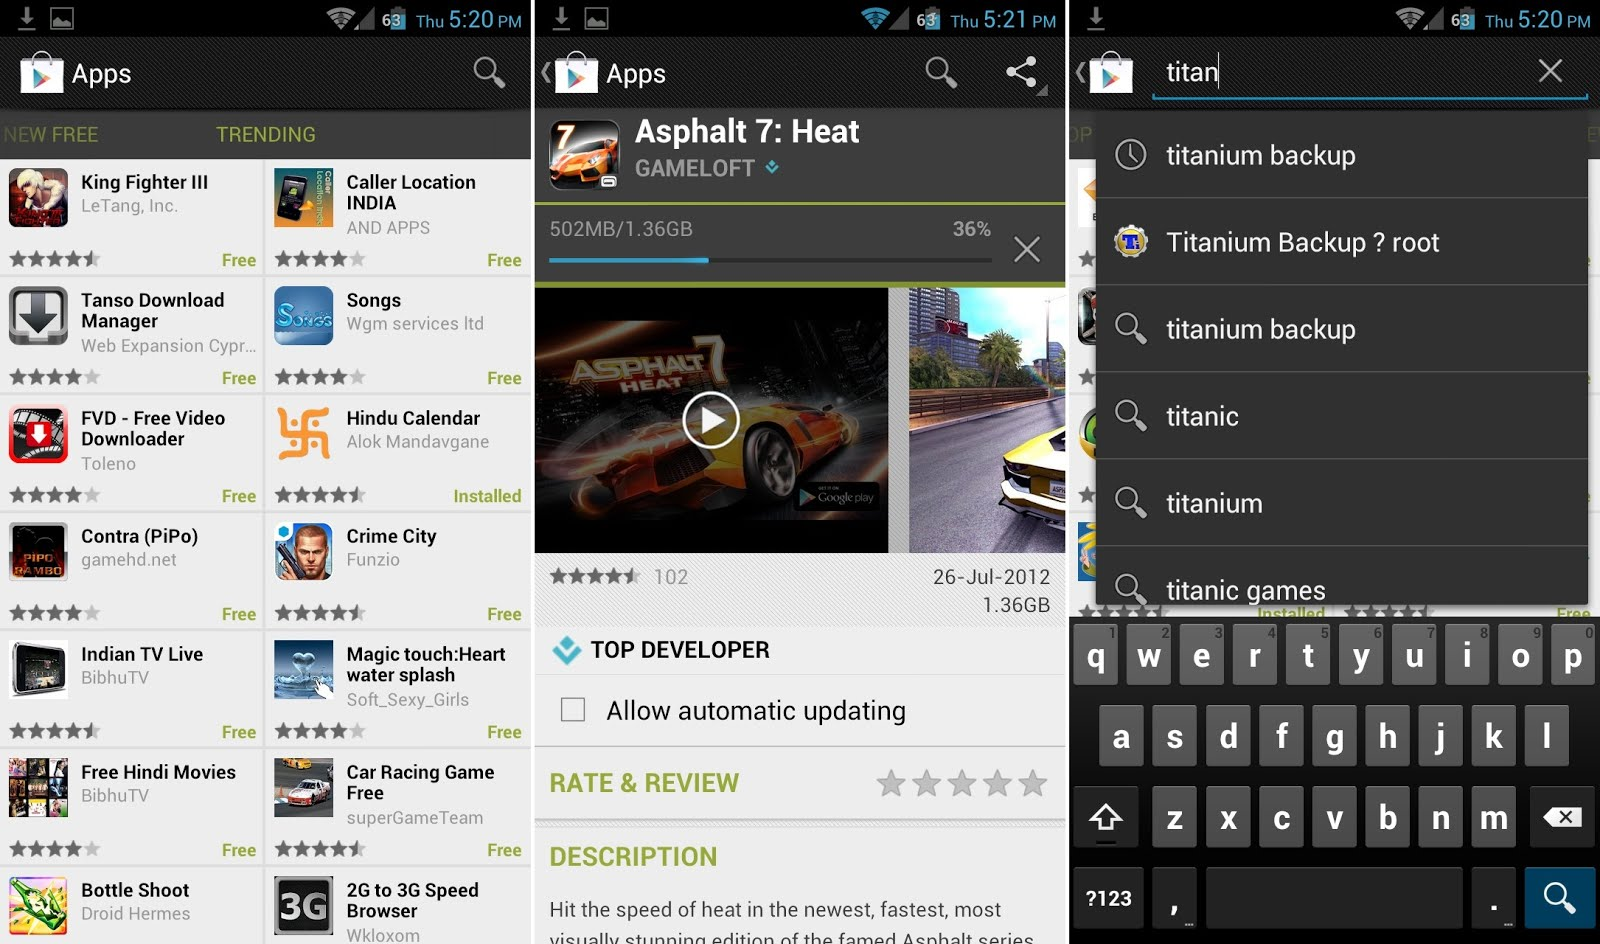
\includegraphics[scale=0.2]{images/Google-Play-Store-APK-3-7-15.jpg}
\caption{Google Play Store}
\end{figure}

{\bf App Store} is also a similar market application, but for apple products\ldots etc\ldots\\
\begin{figure}[H]
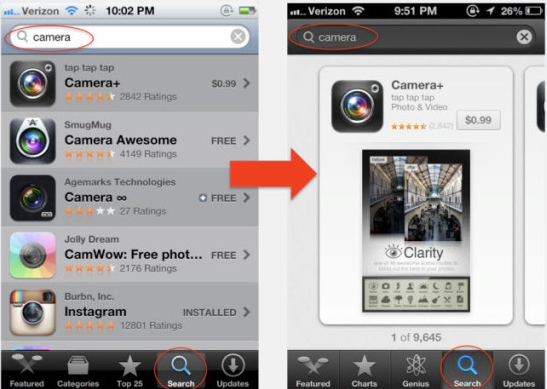
\includegraphics[scale=0.7]{images/png;base642dee0c596030bc1e.png}
\caption{App Store}
\end{figure}
These applications fit the assignment in the way that they are both market applications where one can download applications. This were useful for the development of the product, since it was possible to use the same principles in the assignment. It is also similar in the way that it is possible to browse for applications on the computer, and ''push'' the app to a mobile telephone. This, however, does not connect via bluetooth which the task assignment stated that the finished product should. Based on this, it was not possible to reuse the code or other parts of any of the applications in the development. 

\subsubsection{Over the air transfer}
Pebble is a watch that offers over the air transfer of applications. It is based on the same microchip as one of the newest Arduino\#, but contains an operating system written in C.
\begin{figure}[H]
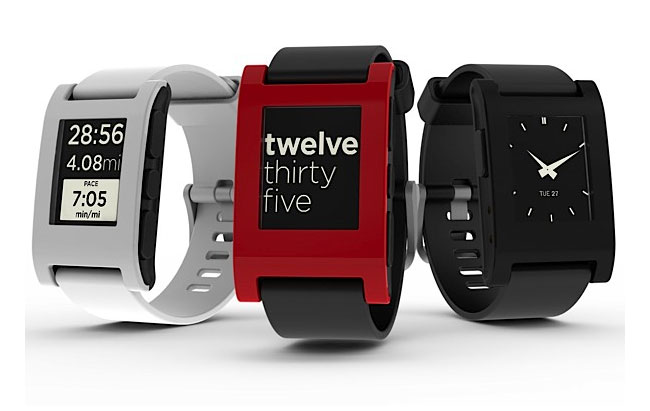
\includegraphics[scale=0.7]{images/Pebble-Smartphone-Watch.jpeg}
\caption{Pebble Watch}
\end{figure}
There is very little documentation on the Pebble website, so the potential reuse in this project appears minimal.